% =============================================================
% Capítulo 4. Desarrollo y resultados
% =============================================================
% Capítulo más extenso. Contenido previsto:
%   - Implementación: arquitectura del sistema
%   - Experimento 1: baseline vs pack-aware (exp02_baseline vs exp03_pack_aware)
%   - Iteración: refinamiento de deck_quality tras saturación
%   - Experimento 2: ejecución con calidad refinada (exp07_run_final, 43 gens)
%   - Exploración descartada: gauntlet tier-1 y sesgo de Forge AI
% =============================================================

\chapter{Evaluación experimental}
\label{cap:desarrollo}

Implementado el sistema, procede ponerlo a prueba. Este capítulo documenta el proceso experimental que validó la propuesta y la evidencia que sostiene cada decisión de diseño. Conviene advertir desde el principio que lo que sigue no es una colección de pruebas independientes, sino un recorrido guiado. Cada experimento responde a una pregunta que planteó el anterior, de acuerdo con la metodología iterativa descrita en el capítulo~\ref{cap:metodologia}. La figura~\ref{fig:recorrido} resume ese recorrido y sirve de mapa para el resto del capítulo.

El punto de partida es un prototipo inicial que, aunque funciona como algoritmo genético, produce mazos poco competitivos (sección~\ref{sec:evolucion}). Su análisis revela cuatro problemas y motiva tres cambios de diseño. El primero de esos experimentos (sección~\ref{sec:experimento-ab}) valida el más importante de los cambios, los operadores pack-aware, mediante una comparativa controlada. Ese experimento destapa a su vez un efecto colateral, ya que la métrica de calidad deja de discriminar entre mazos, lo que obliga a refinarla (sección~\ref{sec:refinamiento}). Con la métrica ya corregida se explora una forma de validar los mazos frente al exterior, un gauntlet de referencias del metajuego real, que finalmente se descarta al detectar un sesgo del simulador (sección~\ref{sec:gauntlet}). Documentar ese límite resulta tan valioso como documentar lo que funciona. Por último, con el sistema ya maduro, se analiza la ejecución más extensa y se comprueba su reproducibilidad con una segunda ejecución independiente (sección~\ref{sec:run-final}).

\begin{figure}[H]
\centering
\begin{tikzpicture}[
    font=\small,
    etapa/.style={draw, rounded corners, align=center, text width=6.2cm, fill=blue!5, inner sep=5pt},
    descartada/.style={draw, rounded corners, align=center, text width=6.2cm, fill=orange!9, inner sep=5pt},
    fl/.style={-{Stealth[length=2.6mm]}, thick}
]
\node[etapa] (proto) {\textbf{Prototipo inicial}\\ mazos poco competitivos (cuatro problemas)};
\node[etapa, below=0.7cm of proto] (ab) {\textbf{Experimento A/B}\\ valida los operadores pack-aware};
\node[etapa, below=0.7cm of ab] (ref) {\textbf{Refinamiento de la métrica}\\ la calidad vuelve a discriminar};
\node[descartada, below=0.7cm of ref] (ga) {\textbf{Gauntlet tier-1} (descartado)\\ sesgo del simulador ante el juego complejo};
\node[etapa, below=0.7cm of ga] (fin) {\textbf{Ejecución final y 2.\textsuperscript{a} ejecución}\\ sistema maduro y reproducible};
\draw[fl] (proto) -- node[right, font=\scriptsize] {tres cambios de diseño} (ab);
\draw[fl] (ab) -- node[right, font=\scriptsize] {la calidad se satura} (ref);
\draw[fl] (ref) -- node[right, font=\scriptsize] {¿validación externa?} (ga);
\draw[fl] (ga) -- node[right, font=\scriptsize] {sistema definitivo} (fin);
\end{tikzpicture}
\caption{Recorrido experimental del capítulo. Cada etapa responde a una pregunta que planteó la anterior, reflejando la metodología iterativa. El prototipo motiva los tres cambios que valida el experimento A/B, cuyo efecto colateral obliga al refinamiento de la métrica. Tras él se explora y se descarta el gauntlet antes de llegar a la ejecución final.}
\label{fig:recorrido}
\vspace{2pt}
{\footnotesize Fuente: elaboración propia.}
\end{figure}

\section{Del prototipo al diseño actual}
\label{sec:evolucion}

El sistema descrito en el capítulo anterior no es el que se construyó al principio. Es el resultado de varias iteraciones, cada una motivada por un problema concreto que la ejecución anterior dejó al descubierto. Conviene examinar esa trayectoria, porque las decisiones de diseño que definen el sistema actual solo se entienden a la luz de lo que vino antes y de por qué no funcionaba.

El primer experimento completo del proyecto evolucionó una población de 20 mazos durante 51 generaciones. La evaluación era round-robin completo: cada mazo jugaba contra los otros 19, lo que sumaba 190 enfrentamientos por generación y un total cercano a los 9700 combates. La ejecución tardó 88 horas, casi cuatro días, en completarse. El fitness combinaba la tasa de victorias y una métrica de calidad con pesos 0.6 y 0.4.

Los resultados confirmaron que el enfoque funcionaba como algoritmo genético (el fitness mejoraba, la élite se preservaba, la población convergía) pero también que los mazos producidos no eran competitivos. El pico de fitness se quedó en 0.791. El mejor mazo del Hall of Fame tenía 39 cartas distintas de 60, es decir, una construcción casi enteramente de copias únicas. Una valoración cualitativa lo situaba en torno a un 3.5 sobre 10 frente a mazos de torneo. Se trataba, en suma, del mejor individuo de una población deficiente.

El diagnóstico identificó cuatro problemas:

\begin{itemize}
    \item El coste de la evaluación crecía con el cuadrado de la población, lo que hacía inviable aumentar el tamaño.
    \item La construcción en copias únicas producía mazos inconsistentes que ningún jugador llevaría a competición.
    \item La función de fitness era demasiado simple.
    \item La población convergía de forma prematura hacia un único par de colores.
\end{itemize}

Los tres últimos problemas comparten una raíz: el algoritmo estaba explorando un espacio de mazos que no se parece al de los mazos competitivos reales. Sobre este diagnóstico se articularon tres cambios de diseño.

El primer cambio abordó el coste. La sustitución del round-robin completo por el Swiss Tournament, descrita en la sección~\ref{sec:torneo}, rompió la dependencia cuadrática con el tamaño de la población. El efecto fue doble. Permitió duplicar la población de 20 a 40 mazos, lo que enriquece la exploración, y aun así redujo el número de enfrentamientos por generación: donde el round-robin habría exigido 780 para 40 mazos, el Swiss exige 160. El cambio no fue solo de eficiencia. El Swiss es el sistema real de los torneos de Magic, de modo que también acercó la evaluación a las condiciones que el trabajo pretende reproducir.

El segundo cambio abordó la irrealidad de los mazos. Los operadores genéticos se reescribieron para trabajar en packs de cuatro copias en lugar de copias sueltas, según el principio de que incluir una carta en un mazo de constructed significa incluir cuatro. Este es el cambio que convierte los mazos de ensamblajes de cartas únicas en construcciones reconocibles, y su validación es el objeto del experimento de la sección~\ref{sec:experimento-ab}. Su efecto medido es una reducción del 95\,\% en los \emph{singletons} sueltos.

El tercer cambio reformuló la función de fitness. El peso del rendimiento en el torneo subió de 0.6 a 0.7, y la métrica de calidad se rediseñó tras detectar que la mejora estructural de los mazos había dejado saturados a varios de sus componentes. Ese refinamiento se detalla en la sección~\ref{sec:refinamiento}.

La diferencia entre el punto de partida y el estado actual es medible en cada dimensión que importaba. El pico de fitness pasó de 0.791 a 0.9755. Los mazos dejaron de ser colecciones de copias únicas para convertirse en construcciones con packs consolidados, manabases coherentes y planes de juego identificables. La población dobló su tamaño sin que el coste por generación se disparara. Además, los mazos del Hall of Fame final contienen cartas reconocibles del meta competitivo de Standard.

El resto del capítulo documenta esa transición con los experimentos que la sostienen. La sección~\ref{sec:experimento-ab} valida el paso a operadores pack-aware con una comparativa controlada. La sección~\ref{sec:refinamiento} detalla el rediseño de la métrica de calidad. La sección~\ref{sec:gauntlet} examina una vía que se exploró y se descartó. La sección~\ref{sec:run-final} analiza la ejecución más extensa con el sistema ya maduro, con el que culmina el capítulo.

\section{Experimento: baseline vs pack-aware}
\label{sec:experimento-ab}

El segundo de los tres cambios de diseño descritos en la sección~\ref{sec:evolucion}, el paso a operadores pack-aware, es el que más afecta a la forma de los mazos. Este experimento lo valida con una comparativa controlada. El experimento examina qué ocurre cuando los operadores genéticos dejan de trabajar en copias sueltas y pasan a operar en packs de cuatro. La hipótesis es que un algoritmo que tome decisiones al nivel en que las toman los jugadores humanos (incluir o excluir una carta como conjunto de cuatro copias) producirá mazos estructuralmente más próximos a los que se juegan en competición. Para validarla se realizaron dos ejecuciones con configuración nominal idéntica. Solo difiere la lógica de variación.

La ejecución de referencia, denominada en adelante \emph{baseline}, usa los operadores originales que modifican copias individuales. La ejecución \emph{pack-aware} sustituye esos operadores por siete operadores temáticos, cada uno modelado sobre una decisión propia de la construcción de mazos: intercambio genérico de cartas, completar packs parciales, ajustar la curva de maná, inyectar respuestas (\emph{removal}), consolidar manabase, mejorar amenazas por coste y reforzar tribus. Ambas corren sobre el mismo catálogo de 4130 cartas.

\subsection{Configuración del experimento}

La tabla~\ref{tab:config-ab} recoge la configuración nominal que comparten las dos ejecuciones, idéntica salvo en la lógica de variación.

\begin{table}[H]
\centering
\caption{Configuración compartida por las dos ejecuciones del experimento A/B.}
\label{tab:config-ab}
\begin{tabular}{lcc}
\toprule
\textbf{Parámetro} & \textbf{Baseline} & \textbf{Pack-aware} \\
\midrule
Población & 40 & 40 \\
Generaciones & 30 & 30 \\
Enfrentamientos por generación & 160 & 160 \\
Selección & Swiss Tournament ($k=8$) & Swiss Tournament ($k=8$) \\
Cuota Hall of Fame por arquetipo & 3 & 3 \\
Conjunto de cartas & 4130 IDs & 4130 IDs \\
Operadores de variación & Copia individual & Pack de 4 copias \\
\bottomrule
\end{tabular}
\\[2pt]{\footnotesize Fuente: elaboración propia.}
\end{table}

El baseline se reanudó una vez: los datos de estadísticas de las generaciones 0-18 no quedaron persistidos en el checkpoint, de modo que solo se dispone de las últimas 12 generaciones (19-30) en los logs de esa ejecución. La ejecución pack-aware corrió de forma continua durante 67.1 horas con 31 generaciones completas y ningún reinicio.

\subsection{Integridad estructural de los mazos}

Antes de comparar el fitness conviene examinar la forma de los mazos que produce cada variante. La tabla~\ref{tab:estructura-ab} reúne las métricas estructurales de la población final en ambas ejecuciones. Los dos cumplen las restricciones formales del formato: los 40 mazos de la población final tienen exactamente 60 cartas y ninguno viola la norma de un máximo de cuatro copias por carta. Hasta ahí llega la equivalencia. A partir de ahí, la diferencia se vuelve pronunciada.

\begin{table}[H]
\centering
\caption{Métricas estructurales de la población final ($n=40$) en ambas ejecuciones.}
\label{tab:estructura-ab}
\begin{tabular}{lcc}
\toprule
\textbf{Métrica} & \textbf{Baseline} & \textbf{Pack-aware} \\
\midrule
Mazos con 60 cartas exactas & 40/40 & 40/40 \\
Violaciones de la norma 4-of & 0 & 0 \\
\emph{Singletons} no-tierra por mazo (media) & 3.55 & 0.17 \\
Sets de 4 copias por mazo (media) & 5.55 & 7.83 \\
Tierras no básicas por mazo (media) & 0.68 & 4.00 \\
Tierras totales por mazo (media) & 20.52 & 25.95 \\
Tasa de fallos en combate & 0.078\,\% & 0.010\,\% \\
\bottomrule
\end{tabular}
\\[2pt]{\footnotesize Fuente: elaboración propia.}
\end{table}

El baseline respeta la norma 4-of en sentido formal: ningún mazo tiene más de cuatro copias de una carta. Pero el espíritu de la norma se viola. Con una media de 3.55 \emph{singletons} no-tierra por mazo, muchos individuos acumulan cinco u ocho cartas en copia única que funcionan como piezas \emph{tech} sueltas (cartas de ajuste puntual, pensadas para situaciones concretas). Los operadores originales, al modificar de copia en copia, generaban y regeneraban esos residuos más rápido de lo que la función de consolidación de \emph{singletons} podía eliminarlos.

En términos concretos, un mazo representativo del baseline podía reunir cuatro copias de dos o tres criaturas centrales y, a su alrededor, una decena larga de cartas en copia única (un hechizo de remoción aquí, un encantamiento allá, una criatura de situación más adelante). Ese repertorio disperso ningún jugador de competición lo registraría, porque diluye el plan de juego y vuelve el mazo inconsistente de una partida a otra: las piezas que deberían definirlo solo aparecen de forma esporádica. El mismo mazo, evolucionado bajo el pack-aware, reemplaza esa dispersión por packs completos de cuatro copias, de modo que las cartas que articulan su estrategia se repiten y comparecen de forma fiable en cada partida.

El pack-aware invierte ese patrón. Los \emph{singletons} no-tierra caen a 0.17 por mazo: prácticamente cero, y los que quedan son residuos legítimos de ajustes de tamaño sobre las tierras, no cartas \emph{tech} dispersas. Los packs consolidados de cuatro copias suben de 5.55 a 7.83 por mazo, un incremento del 41\,\%. Las tierras no básicas pasan de 0.68 a 4.00 por mazo, lo que indica que la manabase empieza a parecerse a la de un mazo competitivo real, con \emph{duals} (tierras que producen dos colores) y tierras de utilidad seleccionadas deliberadamente. En la figura~\ref{fig:estructura} se aprecia el contraste de un vistazo. Las tres magnitudes invierten su relación entre una variante y otra, ya que los \emph{singletons} sueltos, elevados en el baseline, se desploman con el pack-aware, mientras que los packs consolidados y las tierras no básicas, escasos en el baseline, crecen de forma marcada.

\begin{figure}[H]
\centering
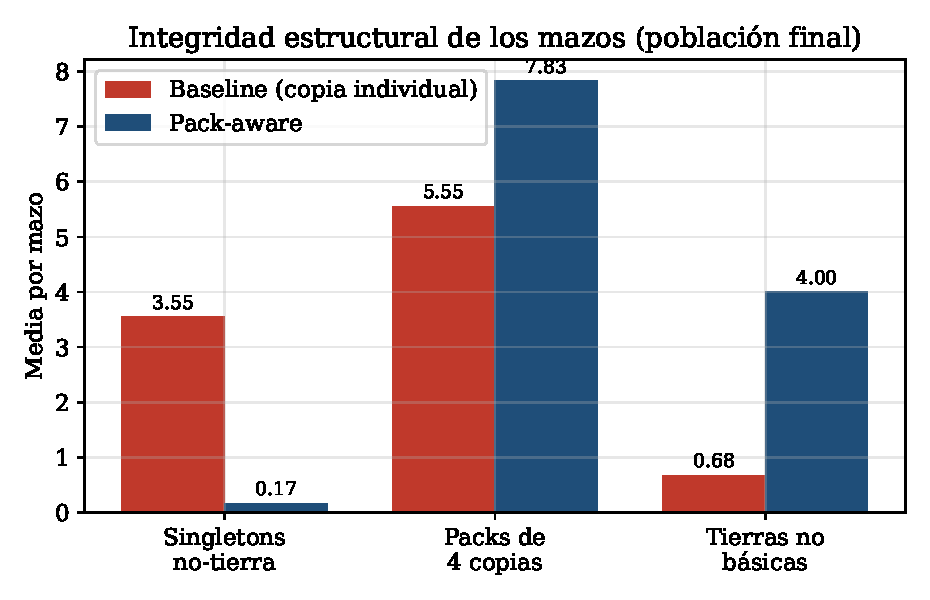
\includegraphics[width=0.78\textwidth]{images/fig_estructura_ab.pdf}
\caption{Métricas estructurales por mazo en la población final, baseline frente a pack-aware. Los \emph{singletons} sueltos se desploman mientras suben los packs consolidados y las tierras no básicas.}
\label{fig:estructura}
\vspace{2pt}{\footnotesize Fuente: elaboración propia.}
\end{figure}

\subsection{Evolución del fitness}

La comparativa anterior muestra que las dos variantes producen mazos de forma muy distinta. Queda por comprobar si esa diferencia estructural se traslada también al rendimiento que mide el fitness. La tabla~\ref{tab:fitness-ab} recoge los estadísticos de fitness de ambas ejecuciones en la ventana de generaciones disponible para las dos.

\begin{table}[H]
\centering
\caption{Estadísticos de fitness comparados. Datos del baseline limitados a las generaciones 19-30 disponibles en sus logs.}
\label{tab:fitness-ab}
\begin{tabular}{lcc}
\toprule
\textbf{Estadístico} & \textbf{Baseline} & \textbf{Pack-aware} \\
\midrule
Pico de \emph{best\_fit} & 0.8906 (gen 29) & 0.8778 (gen 20) \\
\emph{Avg\_fit} en generación final & 0.6171 & 0.6298 \\
\emph{Best\_fit} medio (gens 19-30) & 0.8174 & 0.8200 \\
\emph{Avg\_fit} medio (gens 19-30) & 0.6104 & 0.6256 \\
\bottomrule
\end{tabular}
\\[2pt]{\footnotesize Fuente: elaboración propia.}
\end{table}

Como puede observarse en la tabla, el pico del mejor individuo baja 1.4 puntos porcentuales en la ejecución pack-aware y es, de hecho, el único indicador que retrocede. Por contra, el \emph{avg\_fit} final mejora un 2.1\,\% y la media de \emph{avg\_fit} en la ventana comparable también resulta superior. El diseño pack-aware eleva el rendimiento medio de la población a costa de una ligera reducción en su valor máximo.

La trayectoria interna de la ejecución pack-aware muestra un comportamiento evolutivo adecuado. El \emph{avg\_fit} sube de 0.555 en la generación 0 a 0.630 en la 30, una ganancia del 13.5\,\% con curva sin saltos bruscos. La diversidad estructural de la población cae de 0.878 a 0.396, lo que refleja convergencia progresiva, no colapso súbito. La tasa de mutación adaptativa escaló a 0.9 en las generaciones 14-18 al detectar estancamiento. Esa presión adicional produjo el pico de 0.878 en la generación 20. Las generaciones siguientes relajaron la tasa y no superaron ese pico, aunque el Hall of Fame lo retuvo.

\subsection{Inspección cualitativa del Hall of Fame}

La diferencia más visible entre las dos ejecuciones no reside en las tablas de fitness, sino en la forma de los mazos que produce cada una. A modo de ejemplo, conviene examinar el mejor individuo de cada población. El del baseline es el siguiente:

\begin{center}
\small
\texttt{2 Bake into a Pie, 4 Dawnwing Marshal, 3 Firebrand Archer, 3 Giada,}\\
\texttt{3 Moment of Craving, 2 Mountain, 13 Plains, 5 Swamp, 2 Youthful Valkyrie,}\\
\texttt{3 Anointed Peacekeeper, 1 Flowstone Kavu, 3 Ambush Paratrooper,}\\
\texttt{3 Monastery Swiftspear, 4 Spectrum Sentinel, 1 Survivor of Korlis,}\\
\texttt{2 Warlord's Elite, 1 Axiom Engraver, 2 Infectious Inquiry, 1 Scrollshift,}\\
\texttt{1 Bloodletter of Aclazotz, 1 Lion Heart}
\end{center}

Este mazo contiene tan solo dos packs de cuatro copias y acumula, en cambio, ocho cartas en copia única. Aunque alcanza un fitness de 0.891, ningún jugador de competición lo llevaría a un torneo, ya que se trata de un ensamblaje de piezas que gana partidas en su propio entorno de evaluación (el torneo interno frente al resto de la población), pero que carece de un plan de juego legible.

Por contra, el mejor individuo de la ejecución pack-aware presenta una fisonomía muy distinta:

\begin{center}
\small
\texttt{5 Plains, 17 Swamp, 4 Extinguish the Light, 1 Plaza of Heroes,}\\
\texttt{4 Sheoldred, the Apocalypse, 4 Splatter Goblin, 4 Gurgling Anointer,}\\
\texttt{4 Static Net, 4 Fanatical Offering, 4 Preacher of the Schism,}\\
\texttt{1 Promising Vein, 2 Omenport Vigilante, 1 Fomori Vault,}\\
\texttt{4 Bumbleflower's Sharepot, 1 Maelstrom of the Spirit Dragon}
\end{center}

Este mazo, en cambio, reúne ocho packs de cuatro copias y una manabase con cuatro tierras no básicas de utilidad. Su plan de juego resulta identificable: Sheoldred y Preacher of the Schism actúan como amenazas ganadoras, Extinguish the Light y Static Net aportan las respuestas, y Bumbleflower's Sharepot cumple una función de utilidad. Un jugador humano reconocería esta construcción como un midrange B/W funcional.

El conjunto de \emph{singletons} restantes (Plaza of Heroes, Promising Vein, Fomori Vault, Maelstrom of the Spirit Dragon) corresponde a tierras de utilidad con efecto único, que por su naturaleza se juegan como una o dos copias incluso en los mazos competitivos reales. No son ruido: son decisiones de construcción deliberadas que el pack-aware preserva a través del límite de dos \emph{singletons} que admite la función de corrección.

El resto del Hall of Fame de la ejecución pack-aware muestra el mismo patrón. El mejor control es un B/W con 11 piezas de interacción identificables (Extinguish the Light, Drown in Ichor, Malicious Eclipse) y amenazas tardías. El mejor aggro es un B/G de curva baja con siete packs consolidados y un plan de presión reconocible. Los nueve mazos del Hall of Fame parecen construcciones humanas coherentes.

\subsection{Discusión: la norma de cuatro copias como eje de diseño}

La norma de cuatro copias no es un detalle de implementación. Determina si el algoritmo explora el mismo espacio de configuraciones que recorre un jugador humano o uno esencialmente distinto. En la construcción de mazos de \emph{constructed}, incluir una carta significa incluir cuatro copias: esa es la granularidad mínima con la que razona un jugador. Un operador que modifica copias individuales opera en un espacio de búsqueda que los jugadores humanos nunca recorren.

Los datos del experimento cuantifican el coste y el beneficio de cambiar esa granularidad. El coste es 1.4 puntos porcentuales en el pico de \emph{best\_fit}. El beneficio es una reducción del 95\,\% en \emph{singletons} no-tierra, un incremento del 41\,\% en packs consolidados, y un salto del 488\,\% en tierras no básicas por mazo. El fitness medio de la población sube un 2.1\,\%. La tasa de fallos en combate cae un 87\,\%.

El balance entre coste y beneficio es favorable para el objetivo de este TFG: generar mazos que se parezcan a los que se construyen y juegan en competición. La variante baseline era más explotativa frente a su propio entorno de evaluación, pero sus mazos no serían competitivos fuera de ese contexto. El pack-aware produce mazos menos ajustados al simulador y más próximos al estándar del formato.

El cambio de granularidad también reorienta el arquetipo dominante de la población. En la figura~\ref{fig:arquetipos} puede observarse ese contraste. La población del baseline se concentra en los mazos de agresión, mientras que la del pack-aware se desplaza con claridad hacia el midrange. Ambos resultados son legítimos, pero la convergencia del pack-aware hacia un único arquetipo dominante anticipa el problema de la monocultura que motiva la exploración del gauntlet (sección~\ref{sec:gauntlet}).

\begin{figure}[H]
\centering
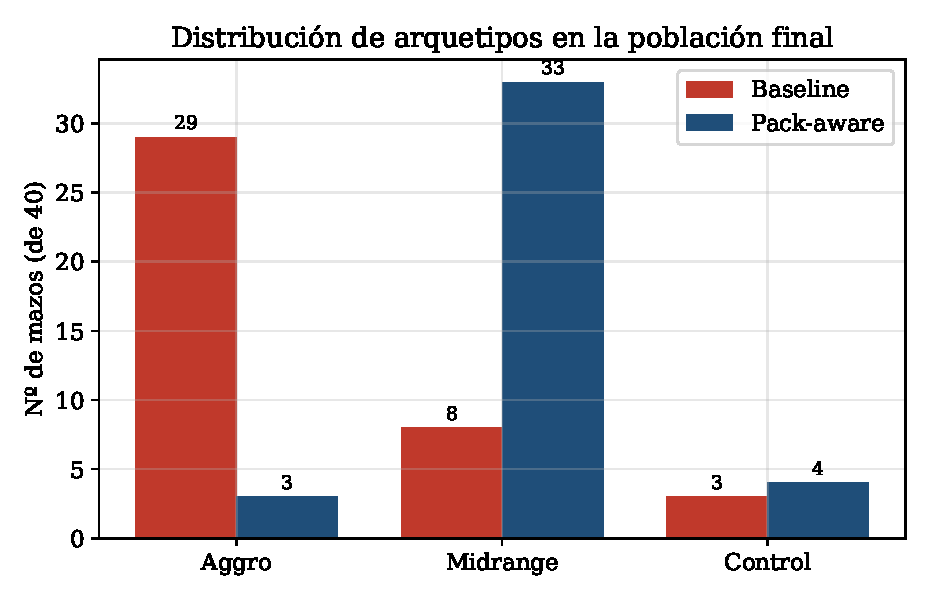
\includegraphics[width=0.72\textwidth]{images/fig_arquetipos_ab.pdf}
\caption{Distribución de arquetipos en la población final de 40 mazos. El baseline está dominado por aggro; el pack-aware, por midrange.}
\label{fig:arquetipos}
\vspace{2pt}{\footnotesize Fuente: elaboración propia.}
\end{figure}

Esta decisión de diseño marca el punto de partida para el resto del desarrollo. Todos los experimentos siguientes asumen operadores pack-aware.

\section{Refinamiento iterativo de la métrica de calidad}
\label{sec:refinamiento}

Cuando el experimento anterior confirmó que los operadores pack-aware funcionaban, apareció un efecto colateral difícil de anticipar: la mejora estructural de los mazos hizo que una parte de la función de fitness dejara de discriminar. El problema es de naturaleza estadística. Se detecta auditando el coeficiente de variación (CoV) de cada componente de la métrica de calidad sobre la población final de la ejecución pack-aware.

\subsection{Diagnóstico: saturación de componentes}

La métrica de calidad combinaba seis componentes con pesos distintos. Antes del pack-aware, esas componentes medían propiedades que podían variar ampliamente de un mazo a otro. Después del pack-aware, tres de ellas convergieron a un valor constante para prácticamente toda la población, como evidencia la tabla~\ref{tab:cov-quality}.

\begin{table}[H]
\centering
\caption{Análisis de varianza de las seis componentes de la métrica de calidad sobre los 40 mazos finales de la ejecución pack-aware (gen 30). CoV $<$ 10\,\% indica saturación.}
\label{tab:cov-quality}
\begin{tabular}{lrrrrl}
\toprule
\textbf{Componente} & \textbf{Peso} & \textbf{Media} & \textbf{StdDev} & \textbf{Rango} & \textbf{CoV} \\
\midrule
Estructura                & 10\,\% & 0.999 & 0.005 & 0.03 & 0.5\,\% \\
Poder de cartas           & 15\,\% & 0.438 & 0.031 & 0.16 & 7.1\,\% \\
Curva de maná             & 20\,\% & 0.835 & 0.064 & 0.28 & 7.7\,\% \\
\midrule
Coherencia de arquetipo   & 15\,\% & 0.886 & 0.153 & 0.51 & 17.3\,\% \\
Sinergia                  & 20\,\% & 0.679 & 0.188 & 0.69 & 27.7\,\% \\
Equilibrio de categorías  & 20\,\% & 0.747 & 0.230 & 0.90 & 30.7\,\% \\
\midrule
\textbf{Calidad (total)} & 100\,\% & 0.751 & 0.087 & 0.32 & 11.6\,\% \\
\bottomrule
\end{tabular}
\\[2pt]{\footnotesize Fuente: elaboración propia.}
\end{table}

Las tres primeras filas son el problema. La estructura mide la proporción de packs consolidados frente a \emph{singletons}: todos los mazos obtienen 0.999 porque el diseño pack-aware garantiza exactamente eso. La curva de maná mide el ajuste de la curva al ideal del arquetipo, pero la función de reparación la regulariza tras cada mutación, por lo que su varianza es trivial. El poder de cartas se saturó por un problema de calibración distinto: toda la población cae en el rango 0.38-0.53, sin gradiente real.

El 45\,\% del peso de la métrica de calidad era, en la práctica, una constante. El CoV total de 11.6\,\% refleja ese ruido: la métrica agregada distingue poco entre un mazo bien construido y uno mediocre. El efecto más visible ocurrió en las primeras ejecuciones con el gauntlet activado: ya en la generación 0 había mazos con fitness 1.0, lo que elimina cualquier gradiente selectivo desde el inicio.

\subsection{Rediseño de la métrica}

La solución al problema de saturación es conceptualmente directa, aunque obliga a decidir qué componentes conservar y con qué peso. Si tres de las seis componentes se han vuelto prácticamente constantes, dejan de aportar información para distinguir un mazo de otro, de modo que carece de sentido que sigan pesando en el agregado. Por ese motivo se eliminan del cálculo de la calidad las tres componentes saturadas, la estructura, el poder de cartas y la curva de maná, y se redistribuye todo su peso entre las tres que sí discriminan. La tabla~\ref{tab:quality-pesos} recoge la ponderación anterior y la nueva.

\begin{table}[H]
\centering
\caption{Ponderación de la métrica de calidad antes y después del refinamiento.}
\label{tab:quality-pesos}
\begin{tabular}{lrrl}
\toprule
\textbf{Componente} & \textbf{Peso anterior} & \textbf{Peso nuevo} & \textbf{Justificación} \\
\midrule
Sinergia                  & 20\,\% & 35\,\% & CoV 27.7\,\%; sinergia interna \\
Equilibrio de categorías  & 20\,\% & 35\,\% & CoV 30.7\,\%; ratio criaturas/hechizos \\
Coherencia de arquetipo   & 15\,\% & 30\,\% & CoV 17.3\,\%; ajuste al arquetipo \\
\midrule
Estructura                & 10\,\% & retirada & saturada \\
Poder de cartas           & 15\,\% & retirada & saturada \\
Curva de maná             & 20\,\% & retirada & saturada \\
\bottomrule
\end{tabular}
\\[2pt]{\footnotesize Fuente: elaboración propia.}
\end{table}

La sinergia y el equilibrio de categorías comparten peso porque sus CoV son equivalentes y miden propiedades ortogonales: la sinergia interna del mazo y el equilibrio entre las categorías de cartas. La coherencia de arquetipo queda un escalón por debajo porque el diseño pack-aware ya fuerza parte de la coherencia arquetípica a través de las cuotas del Hall of Fame. Sigue siendo informativa, aunque es la menos discriminativa de las tres.

Las componentes eliminadas se conservan en la implementación para posibles análisis comparativos futuros. Únicamente se desconectan del agregado.

Con la métrica rediseñada, el peso de la calidad en el fitness se reactivó en $\beta = 0.3$, con lo que la función recupera la forma de la ecuación~\ref{eq:fitness}.

La tasa de victorias del Swiss Tournament sigue siendo el componente principal, que es lo correcto: un mazo que gana partidas pero tiene calidad estructural discreta supera a uno con calidad excelente que pierde. La calidad refinada actúa como desempate entre individuos con una tasa de victorias similar y como ancla que evita que el algoritmo converja hacia mazos con buen rendimiento circunstancial pero incoherentes.

\subsection{Validación del gradiente recuperado}

Para comprobar el efecto del refinamiento se recalcularon las dos versiones de la métrica de calidad sobre los mismos cuarenta mazos de la población final de la ejecución pack-aware que emplea la tabla~\ref{tab:cov-quality}. La métrica original de seis componentes reproduce el diagnóstico previo (media 0.751, CoV 11.4\,\%), lo que valida el procedimiento. La métrica refinada de tres componentes eleva el coeficiente de variación hasta el 19.4\,\% (media 0.765, rango $[0.38,\ 0.91]$): la dispersión relativa casi se duplica, lo que confirma empíricamente que el refinamiento recupera capacidad de discriminación. La media apenas varía, y no desciende como cabría suponer: la eliminación de la componente estructural, saturada en valores altos, se compensa con la del poder de cartas, saturado en valores bajos, de modo que lo que cambia no es el nivel de la métrica, sino su varianza informativa.

El efecto práctico es que el fitness vuelve a tener gradiente en toda la distribución de la población. Dos mazos que empaten en tasa de victorias ya se diferencian por su sinergia interna, por su balance de roles o por su ajuste al arquetipo. Con la métrica de calidad restaurada, el sistema dispone por fin de una función de fitness capaz de ordenar los mazos con finura.

Quedaba, no obstante, un problema de naturaleza distinta que el experimento A/B había dejado abierto, la tendencia de la población a converger hacia una única monocultura cromática. Abordar esa tendencia es el objetivo de la vía que se explora a continuación.

\section{Exploración descartada: gauntlet tier-1}
\label{sec:gauntlet}

Esa tendencia se manifestó con claridad al final de la ejecución pack-aware, donde 37 de los 40 mazos habían convergido al par B/W. Los arquetipos no dominantes sobrevivían únicamente por la cuota del Hall of Fame y no por una presión selectiva real. El diagnóstico es estructural. Cuando la evaluación es puramente intra-poblacional, el arquetipo que mejor rinde contra lo que la propia población produce se autorefuerza hasta desplazar a los demás, de modo que la evaluación acaba premiando la especialización interna en lugar de la competitividad general.

La solución diseñada fue introducir un gauntlet de mazos \emph{tier-1} (de primer nivel competitivo) del metajuego real como componente externo del fitness. Un mazo evolucionado tendría que rendir no solo contra sus compañeros de población, sino contra cinco referencias fijas del metajuego competitivo. Esa presión heterogénea, externa y estable, rompería la retroalimentación que produce la monocultura.

\subsection{Diseño del gauntlet y elección de anchors}

El gauntlet consta de cinco mazos tier-1 del Standard de la era Final Fantasy (junio-julio 2025), elegidos de fuentes públicas (Pro Tour Final Fantasy y MTGGoldfish) para cubrir los grandes arquetipos del meta, según recoge la tabla~\ref{tab:gauntlet-anchors}.

\begin{table}[H]
\centering
\caption{Mazos anchor del gauntlet tier-1, extraídos del meta Standard de junio-julio 2025.}
\label{tab:gauntlet-anchors}
\begin{tabular}{llll}
\toprule
\textbf{Anchor} & \textbf{Arquetipo} & \textbf{Colores} & \textbf{Fuente} \\
\midrule
Izzet Prowess (Baker)   & aggro/combo & U/R & PT Final Fantasy Top 1 \\
Mono-Red Aggro (Fang)   & aggro       & R   & PT Final Fantasy Top 4 \\
Azorius Omniscience     & combo       & U/W & Meta Standard (jul 2025) \\
Dimir Midrange          & midrange    & U/B & Meta Standard (jul 2025) \\
Boros Equipment         & midrange    & R/W & MTGGoldfish (jun 2025) \\
\bottomrule
\end{tabular}
\\[2pt]{\footnotesize Fuente: elaboración propia a partir del Pro Tour Final Fantasy y MTGGoldfish.}
\end{table}

Los cinco anchors son distintos entre sí en colores y estrategia, lo que garantiza que ningún par cromático de la población lo gana todo de entrada. La diversidad del gauntlet es el mecanismo que fuerza diversidad en la población: un mazo aggro R obtendrá buen win-rate contra Azorius pero malo contra Mono-Red; un control U/W hará lo opuesto. El gauntlet presiona en cinco direcciones a la vez.

Con el gauntlet activo, la función de fitness incorpora un tercer término de forma aditiva, como recoge la ecuación~\ref{eq:fitness-gauntlet}.

\begin{equation}
\text{fitness} = \alpha \cdot \text{tasa\_victorias} + \beta \cdot \text{calidad} + \gamma(t) \cdot \text{gauntlet}.
\label{eq:fitness-gauntlet}
\end{equation}

En esta expresión, $\gamma(t)$ crece linealmente de 0.05 en la generación 0 a 0.30 en la última. Este esquema de dificultad creciente, habitual en algoritmos evolutivos, permite que el bloque interno (Swiss + calidad) guíe la exploración inicial, mientras el gauntlet adquiere peso progresivo conforme la población produce candidatos competentes cuya evaluación externa resulta pertinente.

\subsection{Sesgo medible del simulador ante arquetipos de juego complejo}

Dos ejecuciones de validación del gauntlet revelaron un problema que invalida la comparativa externa: el motor Forge aplica la IA del jugador automático con un sesgo sistemático contra arquetipos de juego complejo.

El problema es concreto. Izzet Prowess requiere activar el disparador de \emph{prowess} en el momento exacto del turno del oponente, encadenar hechizos instantáneos en orden preciso y decidir cuándo reservar maná para respuestas. Azorius Omniscience exige secuenciar correctamente la cadena Roiling Dragonstorm / Omniscience y gestionar el maná libre resultante. Forge ejecuta ambas estrategias de forma subóptima: no reconoce las ventanas de juego instantáneo, simplifica las decisiones de encadenamiento y activa triggers en el orden incorrecto.

El efecto sobre el gauntlet es directo. Un mazo evolucionado que enfrente a Izzet Prowess o a Azorius Omniscience no gana porque sea mejor; gana porque su oponente juega por debajo de su potencial real. El win-rate registrado para esos matchups carece de valor discriminativo: cualquier mazo con mínima coherencia superaría esos anchors bajo el Forge AI, independientemente de su calidad real contra versiones jugadas por humanos.

Mono-Red Aggro no tiene este problema: su estrategia es lineal (jugar criaturas baratas, atacar, lanzar daño directo) y Forge la ejecuta razonablemente. Boros Equipment y Dimir Midrange tampoco implican decisiones de alta complejidad en las que el simulador falle de forma sistemática.

El resultado es un gauntlet con tres anchors fiables y dos con sesgo no cuantificable. Bajo esa asimetría, el componente $\gamma \cdot \text{gauntlet}$ introduce ruido en la función de fitness: penaliza correctamente los matchups fiables pero premia artificialmente la derrota de los anchors complejos. El gradiente resultante no mide competitividad real; mide en parte explotación del fallo de la IA.

\subsection{Decisión de descarte}

El gauntlet se descartó como componente del fitness antes de lanzar la ejecución definitiva. La decisión no es de viabilidad técnica: la implementación funciona y los anchors son reproducibles. Es de validez metodológica: incluir un componente de fitness con sesgo conocido y no cuantificable comprometería la interpretabilidad de todos los resultados del TFG.

El problema de la monocultura cromática se abordó de otra forma: la ejecución definitiva, que se analiza en la sección siguiente, se ejecutó sin gauntlet, aceptando que cada ejecución converge a un par cromático y documentando ese comportamiento como un límite del sistema. El ecosistema completo de arquetipos requeriría varias ejecuciones con puntos de partida distintos, lo que se propone como línea de trabajo futuro.

El gauntlet tier-1 queda como exploración válida pero inconclusa. Para activarlo de forma fiable haría falta un motor de simulación con IA más sofisticada, capaz de ejecutar estrategias de juego complejo a nivel competitivo humano. Ese es el bloqueo técnico que la arquitectura actual de Forge no resuelve.

\section{Experimento: ejecución con calidad refinada}
\label{sec:run-final}

Con los operadores pack-aware consolidados, la métrica de calidad rediseñada y descartada la vía del gauntlet, el trabajo culminó con la ejecución más extensa, de la que se extraen las conclusiones principales sobre el comportamiento del sistema. Esta ejecución evolucionó una población de 40 mazos durante 43 generaciones, de la 0 a la 42.

La tabla~\ref{tab:config-final} resume los parámetros con los que se lanzó la ejecución final.

\begin{table}[H]
\centering
\caption{Parámetros de la ejecución final.}
\label{tab:config-final}
\begin{tabular}{ll}
\toprule
\textbf{Parámetro} & \textbf{Valor} \\
\midrule
Población & 40 mazos \\
Generaciones & 43 (gen 0 a gen 42) \\
Enfrentamientos por generación & 160 \\
Selección & Swiss Tournament ($k=8$) \\
Cuota Hall of Fame por arquetipo & 3 \\
Operadores de variación & Pack-aware (7 operadores) \\
Fitness & $0.7 \cdot \text{tasa\_victorias} + 0.3 \cdot \text{calidad}$ \\
Conjunto de cartas & 4130 IDs \\
\bottomrule
\end{tabular}
\\[2pt]{\footnotesize Fuente: elaboración propia.}
\end{table}

La tabla~\ref{tab:fitness-final} recoge los estadísticos de fitness en generaciones representativas de la ejecución final.

\begin{table}[H]
\centering
\caption{Estadísticos de fitness en generaciones representativas de la ejecución final.}
\label{tab:fitness-final}
\begin{tabular}{rrrrr}
\toprule
\textbf{Gen} & \textbf{best\_fit} & \textbf{avg\_fit} & \textbf{diversidad} & \textbf{mut\_rate} \\
\midrule
0  & 0.8401 & 0.5268 & 0.871 & 0.60 \\
5  & 0.8382 & 0.5220 & 0.762 & 0.60 \\
10 & 0.8734 & 0.5256 & 0.735 & 0.75 \\
15 & 0.8828 & 0.5371 & 0.562 & 0.90 \\
18 & 0.9427 & 0.5372 & 0.586 & 0.90 \\
22 & 0.9427 & 0.5610 & 0.541 & 0.60 \\
30 & 0.9045 & 0.5693 & 0.418 & 0.90 \\
38 & 0.9475 & 0.5696 & 0.477 & 0.90 \\
\textbf{42} & \textbf{0.9755} & \textbf{0.5983} & \textbf{0.438} & \textbf{0.60} \\
\bottomrule
\end{tabular}
\\[2pt]{\footnotesize Fuente: elaboración propia.}
\end{table}

El \emph{avg\_fit} sube de 0.527 en la generación 0 a 0.598 en la generación 42, un incremento del 13.5\,\%. La trayectoria es ascendente y sin saltos bruscos, lo que descarta convergencia prematura. El primer salto significativo del \emph{best\_fit} ocurre en la generación 18, donde la tasa de mutación adaptativa lleva varios ciclos a 0.9 para romper un estancamiento. Ese esfuerzo produce el primer pico de 0.9427. Generaciones posteriores consolidan esa ganancia sin retroceder por debajo de 0.88.

El pico absoluto, 0.9755, aparece en la generación 42, la última de la ejecución. Ese dato admite una lectura favorable: el mejor individuo aún mejoraba en el momento de la terminación, lo que sugiere que el proceso no había agotado su margen de mejora. Hasta dónde podría llegar con más generaciones es, no obstante, algo que solo una ejecución más prolongada permitiría determinar. En la figura~\ref{fig:fitness} se aprecia con claridad esta dinámica. La curva del mejor individuo oscila de forma acusada de una generación a otra, reflejo del ruido de la evaluación por simulación, mientras que la curva de la media de la población asciende de manera sostenida y sin retrocesos. Ese ascenso continuo de la media, y no solo del máximo, es lo que confirma que la mejora es poblacional y no obra de un único individuo afortunado.

\begin{figure}[H]
\centering
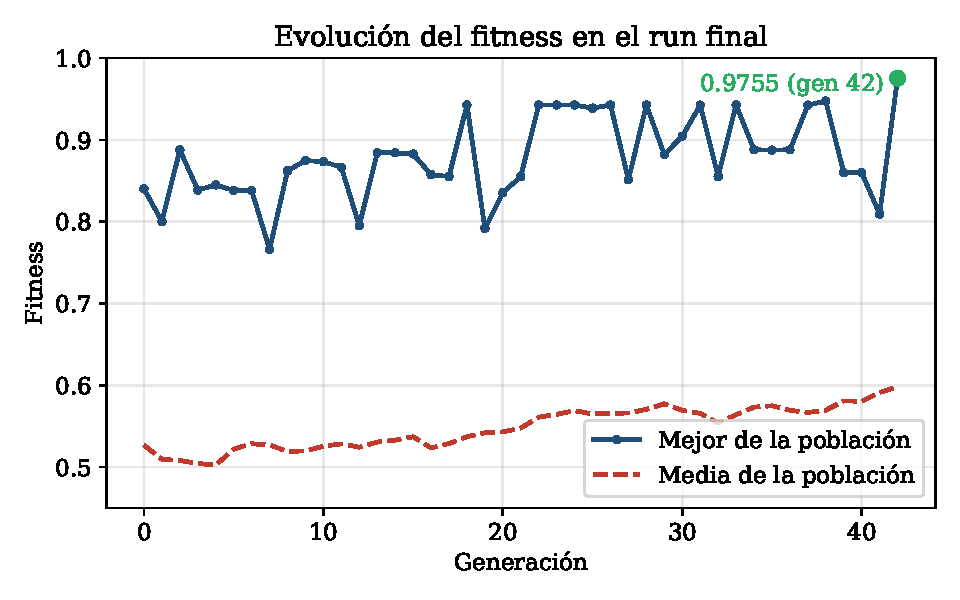
\includegraphics[width=0.82\textwidth]{images/fig_evolucion_fitness.pdf}
\caption{Evolución del fitness de la ejecución final. El mejor de cada generación fluctúa por el ruido de la evaluación por simulación, mientras la media asciende de forma sostenida. El pico de 0.9755 se alcanza en la última generación.}
\label{fig:fitness}
\vspace{2pt}{\footnotesize Fuente: elaboración propia.}
\end{figure}

La diversidad estructural cae de 0.871 a 0.438 a lo largo de la ejecución, lo que responde a una convergencia natural, ya que la población se especializa en torno al par cromático dominante sin llegar a colapsar. La entropía de arquetipo en la generación 42 es 0.715, un nivel que indica coexistencia real de aggro, midrange y control en el Hall of Fame, aunque con pesos desiguales. La figura~\ref{fig:dinamica} reúne las tres magnitudes que describen esa dinámica. Como puede observarse, la diversidad estructural y la entropía de arquetipo descienden de forma paralela conforme la población se especializa, mientras que la tasa de mutación adaptativa dibuja un perfil escalonado, con picos hasta 0.9 en los tramos de estancamiento que fuerzan la exploración y descensos en las fases de consolidación. La lectura conjunta muestra un sistema que alterna exploración y explotación de forma autorregulada.

\begin{figure}[H]
\centering
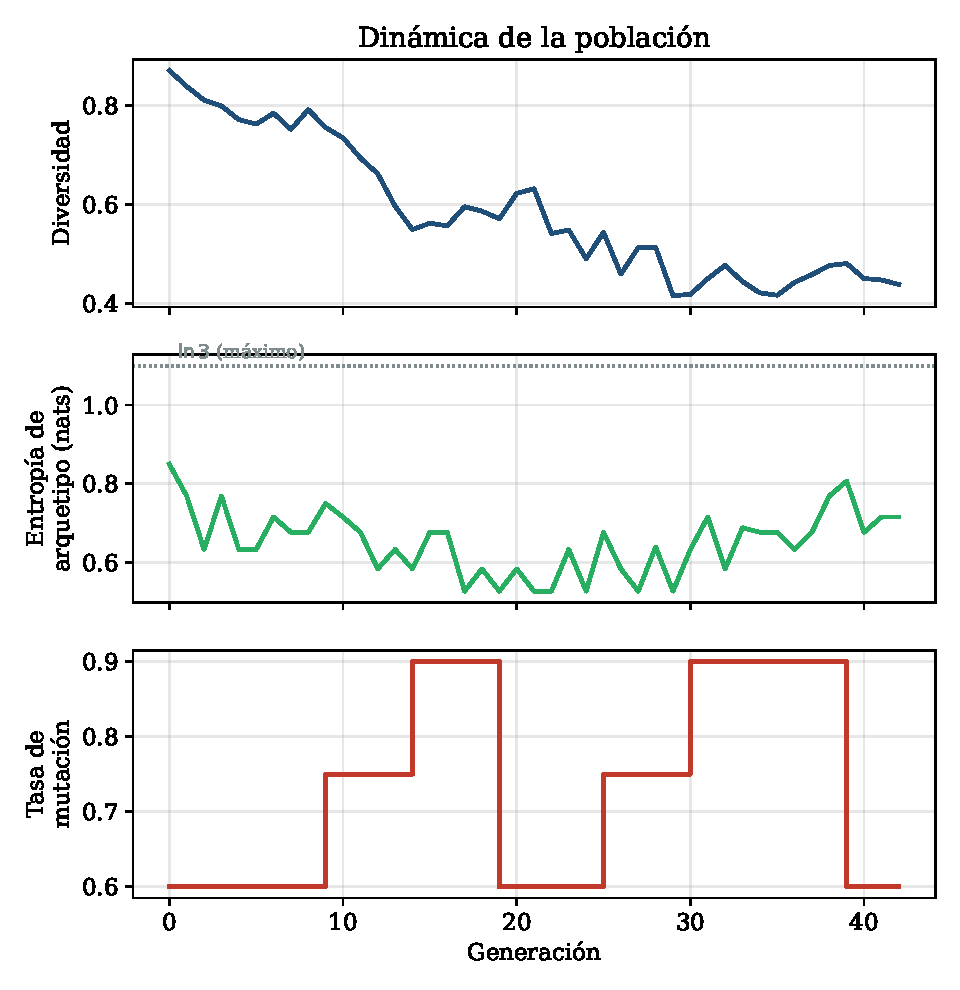
\includegraphics[width=0.78\textwidth]{images/fig_dinamica_poblacion.pdf}
\caption{Dinámica de la población. La diversidad y la entropía de arquetipo descienden conforme la población se especializa. La tasa de mutación sube a 0.9 en los tramos de estancamiento para forzar exploración.}
\label{fig:dinamica}
\vspace{2pt}{\footnotesize Fuente: elaboración propia.}
\end{figure}

\subsection{Atractor cromático: R/W Boros}

Cada ejecución del algoritmo converge a un único par cromático. La ejecución final converge a R/W (Boros). Este es el comportamiento esperado: la presión selectiva favorece mazos coherentes con una manabase de dos colores, y el primer par que consigue ese nivel de coherencia atrae las mutaciones sucesivas hacia sí mismo. Los tres mejores mazos del Hall of Fame, uno de cada arquetipo, son Boros:

\begin{itemize}
    \item \textbf{Aggro R/W}: curva baja con Scalestorm Summoner, Inti, Seneschal of the Sun, Werefox Bodyguard y Roc Hunter como núcleo de amenazas.
    \item \textbf{Midrange R/W}: Leyline Axe, Giant Cindermaw, Defiler of Instinct y Buster Sword como paquete de presión mediada con tierras de utilidad (Temple of Triumph, Crawling Barrens).
    \item \textbf{Control R/W}: Scalestorm Summoner como \emph{win condition} (la carta encargada de cerrar la partida) en el juego tardío, Volt Charge, Galvanize, Flame Lash y Twin Bolt como conjunto de remoción de daño, Dragon Fodder como generación de fichas (\emph{tokens}).
\end{itemize}

Leyline Axe y Scalestorm Summoner aparecen en dos de los tres mazos del Hall of Fame, lo que señala que el algoritmo identificó esas cartas como piezas de alto valor en el contexto cromático convergido. Ambas son cartas del metajuego competitivo de Standard.

\subsection{Inspección del Hall of Fame final}

El mazo con la fitness más alta del Hall of Fame, y por tanto el campeón de la ejecución, es el R/W con 0.9755 que el detector de arquetipos clasifica como control:

\begin{center}
\small
\texttt{4 Dragon Fodder, 4 Leyline Axe, 4 Scalestorm Summoner, 4 Volt Charge,}\\
\texttt{4 Galvanize, 4 Flame Lash, 4 Twin Bolt, 2 Defiler of Instinct,}\\
\texttt{3 Dragonwing Glider, 2 Monument to Perfection,}\\
\texttt{20 Mountain, 2 Plains, 1 Temple of Triumph, 1 Crawling Barrens, 1 Capital City}
\end{center}

Este mazo se articula en siete packs de cuatro copias y 25 tierras. Su núcleo es un paquete de quemado denso, ya que Volt Charge, Galvanize, Flame Lash y Twin Bolt suman dieciséis cartas de daño directo, respaldadas por Scalestorm Summoner como amenaza recurrente y por Dragon Fodder como generación de fichas, mientras que Leyline Axe aporta presión equipada. Con solo seis criaturas y un coste de maná medio de 3.06, la heurística lo etiqueta como control, aunque funcionalmente es un mazo de quemado agresivo. Esa discrepancia entre el arquetipo detectado y el plan de juego real ilustra el límite de una detección basada únicamente en coste medio y número de criaturas. En la figura~\ref{fig:curvamana} se observa su curva de maná. La mayor parte de las cartas se concentra en los costes de dos a cuatro de maná, sin apenas presencia por encima, un perfil bajo y comprimido que es justamente el que exige un plan de quemado agresivo, orientado a cerrar la partida antes de que el coste de las cartas se convierta en un lastre.

\begin{figure}[H]
\centering
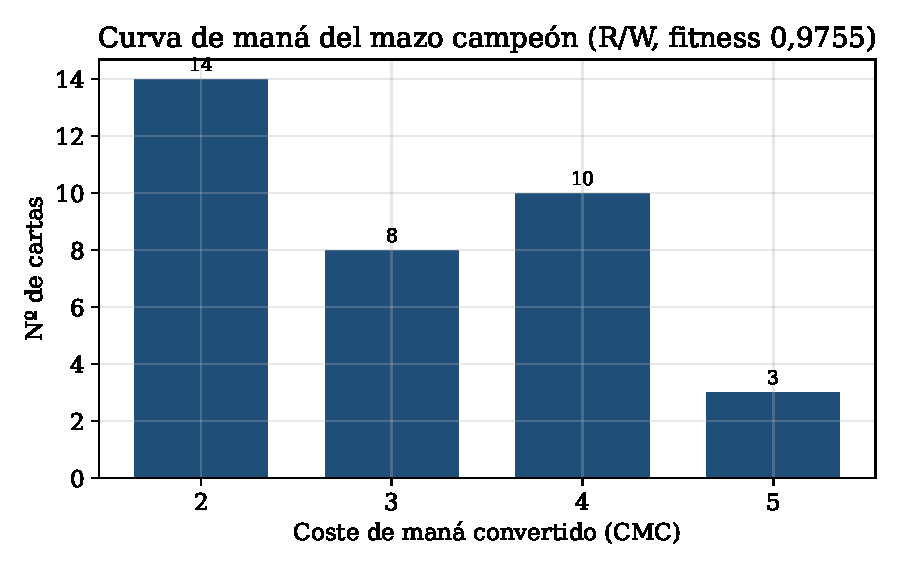
\includegraphics[width=0.66\textwidth]{images/fig_curva_mana_campeon.pdf}
\caption{Curva de maná de las cartas no-tierra del mazo campeón. La concentración en costes de dos a cuatro maná refleja un plan de juego agresivo basado en daño directo.}
\label{fig:curvamana}
\vspace{2pt}{\footnotesize Fuente: elaboración propia.}
\end{figure}

La calidad del mazo campeón admite una lectura desde tres perspectivas complementarias. En el plano cuantitativo, alcanza el fitness más alto de la ejecución, 0.9755, que integra tanto su tasa de victorias en el torneo como su calidad estructural. En el plano de la composición, converge al par cromático Boros (R/W), que coincide con el de arquetipos competitivos vigentes del formato, como los mazos de tipo Boros Equipment, y reúne cartas presentes en el metajuego de Standard. Desde una valoración cualitativa del autor, con experiencia en el formato, el mazo exhibe un plan de quemado coherente, una base de tierras funcional y una curva concentrada en costes bajos y medios. Un jugador reconocería la construcción como apta para competición sin necesidad de cambios estructurales. Una validación externa más exigente, que enfrentara el mazo a referencias del metajuego real, queda condicionada por el sesgo del simulador ante los arquetipos de mayor complejidad táctica, y se plantea como línea de trabajo futuro.


\subsection{Una segunda ejecución independiente}
\label{sec:repro}

Todos los resultados anteriores proceden de una sola ejecución. Para disponer de una primera comprobación de reproducibilidad, se realizó una segunda ejecución con una configuración \emph{idéntica} a la de la ejecución final (población de 40 mazos, Swiss con $k=8$, fitness $0.7\cdot\text{tasa\_victorias}+0.3\cdot\text{calidad}$ y sin gauntlet). La única diferencia es el punto de partida: el sistema no fija la semilla del generador aleatorio, de modo que cada ejecución genera su propia población inicial de 40 mazos y toma decisiones aleatorias independientes. Ambas ejecuciones son, por tanto, réplicas independientes que arrancan de mazos distintos.

La tabla~\ref{tab:dos-ejecuciones} contrasta las dos. La segunda ejecución evolucionó durante 37 generaciones y alcanzó un pico de fitness de 0.9651 en la última, con un fitness medio que creció un 10.6\,\%. Su población no convergió al par rojo-blanco de la ejecución final, sino a un mazo \emph{midrange} monocolor blanco, articulado en torno a criaturas eficientes, remoción y varias copias del planeswalker Elspeth, Storm Slayer.

\begin{table}[H]
\centering
\caption{Comparación de las dos ejecuciones independientes con el sistema definitivo. La configuración nominal es idéntica. Solo difieren la población inicial aleatoria y el azar de la evolución.}
\label{tab:dos-ejecuciones}
\begin{tabular}{lcc}
\toprule
\textbf{Métrica} & \textbf{Ejecución final} & \textbf{2.\textsuperscript{a} ejecución} \\
\midrule
Generaciones & 43 & 37 \\
Pico de fitness (última gen.) & 0.9755 & 0.9651 \\
Incremento del fitness medio & +13.5\,\% & +10.6\,\% \\
Par cromático convergido & R/W (Boros) & Mono-blanco (W) \\
Arquetipo del campeón & Quemado agresivo & Midrange \\
\bottomrule
\end{tabular}
\\[2pt]{\footnotesize Fuente: elaboración propia.}
\end{table}

De esta comparación se extraen dos observaciones. La primera es que la convergencia a un único par cromático no es un artefacto de una ejecución concreta: las dos ejecuciones, partiendo de poblaciones iniciales distintas, convergieron cada una a un par de colores, y esos pares fueron diferentes (rojo-blanco frente a monocolor blanco). Este comportamiento respalda tanto la hipótesis de la convergencia cromática como la idea de que el sistema, a lo largo de varias ejecuciones, exploraría un ecosistema de arquetipos en lugar de una única solución. La segunda es que el pico de fitness es estable entre ejecuciones: 0.9755 y 0.9651 sitúan el rendimiento máximo en torno a 0.97 en ambos casos, lo que indica que ese nivel no depende de una semilla afortunada.

El mazo campeón de esta segunda ejecución, con fitness 0.9651, es el siguiente:

\begin{center}
\small
\texttt{4 Leonin Skyhunter, 3 Coppercoat Vanguard, 1 Inspiring Paladin,}\\
\texttt{4 Sundial Dawn Tyrant, 4 Sage of the Skies, 4 Oltec Cloud Guard,}\\
\texttt{4 Rosa Resolute White Mage, 4 Elspeth Storm Slayer,}\\
\texttt{1 Celestial Armor, 4 Soul Partition, 4 Split Up,}\\
\texttt{18 Plains, 1 The Seedcore, 1 Echoing Deeps, 1 Bucolic Ranch,}\\
\texttt{1 Tarnation Vista, 1 Fountainport}
\end{center}

Al igual que el campeón Boros, es una construcción coherente y reconocible. Reúne ocho packs de cuatro copias y exhibe un plan de juego legible: una base de criaturas blancas eficientes (Leonin Skyhunter, Coppercoat Vanguard o Sundial Dawn Tyrant) sostiene la presión en los primeros turnos. Soul Partition y Split Up aportan la interacción, puntual y en barrido, mientras que los cuatro ejemplares de Elspeth, Storm Slayer actúan como remate y motor de ventaja de cartas. Con veintitrés tierras y un coste de maná medio de 3.03, la curva se concentra en los costes de dos a cuatro maná (quince, diez y ocho cartas, respectivamente) y culmina en el cinco de Elspeth, un perfil propio de un midrange agresivo que un jugador reconocería como un mazo mono-blanco de competición.

Que dos ejecuciones independientes produzcan cada una un campeón estructuralmente coherente, pero de colores y plan de juego distintos, refuerza que el sistema no encuentra un único mazo afortunado, sino construcciones viables en más de un punto del espacio de arquetipos.

Conviene, no obstante, acotar el alcance de esta comprobación. Dos ejecuciones constituyen una muestra reducida: sostienen la reproducibilidad del comportamiento observado, pero no equivalen a una validación estadística, que requeriría un mayor número de repeticiones. Además, al no fijarse la semilla, ninguna de las dos ejecuciones es reproducible de forma exacta. Un barrido controlado de semillas, planteado entre las líneas de trabajo futuro, permitiría cuantificar con rigor la variabilidad del método.
